\documentclass[twoside]{book}

% Packages required by doxygen
\usepackage{fixltx2e}
\usepackage{calc}
\usepackage{doxygen}
\usepackage[export]{adjustbox} % also loads graphicx
\usepackage{graphicx}
\usepackage[utf8]{inputenc}
\usepackage{makeidx}
\usepackage{multicol}
\usepackage{multirow}
\PassOptionsToPackage{warn}{textcomp}
\usepackage{textcomp}
\usepackage[nointegrals]{wasysym}
\usepackage[table]{xcolor}

% Font selection
\usepackage[T1]{fontenc}
\usepackage[scaled=.90]{helvet}
\usepackage{courier}
\usepackage{amssymb}
\usepackage{sectsty}
\renewcommand{\familydefault}{\sfdefault}
\allsectionsfont{%
  \fontseries{bc}\selectfont%
  \color{darkgray}%
}
\renewcommand{\DoxyLabelFont}{%
  \fontseries{bc}\selectfont%
  \color{darkgray}%
}
\newcommand{\+}{\discretionary{\mbox{\scriptsize$\hookleftarrow$}}{}{}}

% Page & text layout
\usepackage{geometry}
\geometry{%
  a4paper,%
  top=2.5cm,%
  bottom=2.5cm,%
  left=2.5cm,%
  right=2.5cm%
}
\tolerance=750
\hfuzz=15pt
\hbadness=750
\setlength{\emergencystretch}{15pt}
\setlength{\parindent}{0cm}
\setlength{\parskip}{3ex plus 2ex minus 2ex}
\makeatletter
\renewcommand{\paragraph}{%
  \@startsection{paragraph}{4}{0ex}{-1.0ex}{1.0ex}{%
    \normalfont\normalsize\bfseries\SS@parafont%
  }%
}
\renewcommand{\subparagraph}{%
  \@startsection{subparagraph}{5}{0ex}{-1.0ex}{1.0ex}{%
    \normalfont\normalsize\bfseries\SS@subparafont%
  }%
}
\makeatother

% Headers & footers
\usepackage{fancyhdr}
\pagestyle{fancyplain}
\fancyhead[LE]{\fancyplain{}{\bfseries\thepage}}
\fancyhead[CE]{\fancyplain{}{}}
\fancyhead[RE]{\fancyplain{}{\bfseries\leftmark}}
\fancyhead[LO]{\fancyplain{}{\bfseries\rightmark}}
\fancyhead[CO]{\fancyplain{}{}}
\fancyhead[RO]{\fancyplain{}{\bfseries\thepage}}
\fancyfoot[LE]{\fancyplain{}{}}
\fancyfoot[CE]{\fancyplain{}{}}
\fancyfoot[RE]{\fancyplain{}{\bfseries\scriptsize Generated by Doxygen }}
\fancyfoot[LO]{\fancyplain{}{\bfseries\scriptsize Generated by Doxygen }}
\fancyfoot[CO]{\fancyplain{}{}}
\fancyfoot[RO]{\fancyplain{}{}}
\renewcommand{\footrulewidth}{0.4pt}
\renewcommand{\chaptermark}[1]{%
  \markboth{#1}{}%
}
\renewcommand{\sectionmark}[1]{%
  \markright{\thesection\ #1}%
}

% Indices & bibliography
\usepackage{natbib}
\usepackage[titles]{tocloft}
\setcounter{tocdepth}{3}
\setcounter{secnumdepth}{5}
\makeindex

% Hyperlinks (required, but should be loaded last)
\usepackage{ifpdf}
\ifpdf
  \usepackage[pdftex,pagebackref=true]{hyperref}
\else
  \usepackage[ps2pdf,pagebackref=true]{hyperref}
\fi
\hypersetup{%
  colorlinks=true,%
  linkcolor=blue,%
  citecolor=blue,%
  unicode%
}

% Custom commands
\newcommand{\clearemptydoublepage}{%
  \newpage{\pagestyle{empty}\cleardoublepage}%
}

\usepackage{caption}
\captionsetup{labelsep=space,justification=centering,font={bf},singlelinecheck=off,skip=4pt,position=top}

%===== C O N T E N T S =====

\begin{document}

% Titlepage & ToC
\hypersetup{pageanchor=false,
             bookmarksnumbered=true,
             pdfencoding=unicode
            }
\pagenumbering{alph}
\begin{titlepage}
\vspace*{7cm}
\begin{center}%
{\Large E-\/\+Classroom Display Server \\[1ex]\large 1 }\\
\vspace*{1cm}
{\large Generated by Doxygen 1.8.13}\\
\end{center}
\end{titlepage}
\clearemptydoublepage
\pagenumbering{roman}
\tableofcontents
\clearemptydoublepage
\pagenumbering{arabic}
\hypersetup{pageanchor=true}

%--- Begin generated contents ---
\chapter{E-\/\+Classroom Display server}
\label{index}\hypertarget{index}{}\begin{DoxyAuthor}{Author}
Rick Ovehorst, Gerjon Eilander \& Gerben van \textquotesingle{}t Ooster 
\end{DoxyAuthor}
\begin{DoxyVersion}{Version}
1.\+0 
\end{DoxyVersion}
\hypertarget{index_intro_sec}{}\section{Introduction}\label{index_intro_sec}
This server program sends schedule data from the Windesheim\textquotesingle{}s systems to the modules upon request.\hypertarget{index_compile_sec}{}\section{Using the software}\label{index_compile_sec}
\hypertarget{index_install}{}\subsection{neccesary packages}\label{index_install}
The packages that are neccesary, can be optained by using folowing commands \+: 
\begin{DoxyCode}
sudo apt-\textcolor{keyword}{get} install libmysqlclient-dev
sudo apt-\textcolor{keyword}{get} install libcurl4-nss-dev 
sudo apt-\textcolor{keyword}{get} install libjsoncpp-nss-dev
sudo apt-\textcolor{keyword}{get} install mysql-\hyperlink{main_8h_afd1a82c786509e03b540bae82af2c137}{server}
sudo apt-\textcolor{keyword}{get} install mysql-client
\end{DoxyCode}


Packages neccesary for compiling\+: 
\begin{DoxyCode}
sudo apt-\textcolor{keyword}{get} install gcc
sudo apt-\textcolor{keyword}{get} install make
\end{DoxyCode}
\hypertarget{index_run}{}\subsection{Running the software}\label{index_run}
To run the software use the following command\+: sudo bin/server $<$ip$>$ $<$port$>$ 
\chapter{Class Index}
\section{Class List}
Here are the classes, structs, unions and interfaces with brief descriptions\+:\begin{DoxyCompactList}
\item\contentsline{section}{\hyperlink{classCurlHandler}{Curl\+Handler} }{\pageref{classCurlHandler}}{}
\item\contentsline{section}{\hyperlink{classECDH}{E\+C\+DH} }{\pageref{classECDH}}{}
\item\contentsline{section}{\hyperlink{classMysqlHandler}{Mysql\+Handler} }{\pageref{classMysqlHandler}}{}
\item\contentsline{section}{\hyperlink{classServer}{Server} }{\pageref{classServer}}{}
\end{DoxyCompactList}

\chapter{File Index}
\section{File List}
Here is a list of all files with brief descriptions\+:\begin{DoxyCompactList}
\item\contentsline{section}{/home/rso16/projects/\+E\+C\+D\+S/src/\hyperlink{main_8cpp}{main.\+cpp} }{\pageref{main_8cpp}}{}
\item\contentsline{section}{/home/rso16/projects/\+E\+C\+D\+S/src/\hyperlink{main_8h}{main.\+h} }{\pageref{main_8h}}{}
\item\contentsline{section}{/home/rso16/projects/\+E\+C\+D\+S/src/\+Curl\+Handler/\hyperlink{CurlHandler_8cpp}{Curl\+Handler.\+cpp} }{\pageref{CurlHandler_8cpp}}{}
\item\contentsline{section}{/home/rso16/projects/\+E\+C\+D\+S/src/\+Curl\+Handler/\hyperlink{CurlHandler_8h}{Curl\+Handler.\+h} }{\pageref{CurlHandler_8h}}{}
\item\contentsline{section}{/home/rso16/projects/\+E\+C\+D\+S/src/\+E\+C\+D\+H/\hyperlink{ECDH_8cpp}{E\+C\+D\+H.\+cpp} }{\pageref{ECDH_8cpp}}{}
\item\contentsline{section}{/home/rso16/projects/\+E\+C\+D\+S/src/\+E\+C\+D\+H/\hyperlink{ECDH_8h}{E\+C\+D\+H.\+h} }{\pageref{ECDH_8h}}{}
\item\contentsline{section}{/home/rso16/projects/\+E\+C\+D\+S/src/\+Mysql\+Handler/\hyperlink{MysqlHandler_8cpp}{Mysql\+Handler.\+cpp} }{\pageref{MysqlHandler_8cpp}}{}
\item\contentsline{section}{/home/rso16/projects/\+E\+C\+D\+S/src/\+Mysql\+Handler/\hyperlink{MysqlHandler_8h}{Mysql\+Handler.\+h} }{\pageref{MysqlHandler_8h}}{}
\item\contentsline{section}{/home/rso16/projects/\+E\+C\+D\+S/src/\+Server/\hyperlink{Server_8cpp}{Server.\+cpp} }{\pageref{Server_8cpp}}{}
\item\contentsline{section}{/home/rso16/projects/\+E\+C\+D\+S/src/\+Server/\hyperlink{Server_8h}{Server.\+h} }{\pageref{Server_8h}}{}
\end{DoxyCompactList}

\chapter{Class Documentation}
\hypertarget{classCurlHandler}{}\section{Curl\+Handler Class Reference}
\label{classCurlHandler}\index{Curl\+Handler@{Curl\+Handler}}


{\ttfamily \#include $<$Curl\+Handler.\+h$>$}

\subsection*{Public Member Functions}
\begin{DoxyCompactItemize}
\item 
char $\ast$ \hyperlink{classCurlHandler_a8f82086fdc6993eb9068a25632652fb0}{get\+Lesson\+Info} (int class\+Id)
\begin{DoxyCompactList}\small\item\em This function retrieves \& parses json  none. \end{DoxyCompactList}\item 
std\+::string \hyperlink{classCurlHandler_a3b115e8ef11a96743b49797b4025b3a0}{curl\+Request} (int ID)
\begin{DoxyCompactList}\small\item\em This function requests Room data from roostertest.\+windesheim.\+nl by Room\+ID.  none. \end{DoxyCompactList}\item 
std\+::string \hyperlink{classCurlHandler_a967784524e6d6d95b1d7089e3221fbfb}{get\+Curl\+U\+RL} (int ID)
\begin{DoxyCompactList}\small\item\em This function creates the curl request U\+RL with Date \& Room\+ID.  String of U\+RL. \end{DoxyCompactList}\item 
std\+::string \hyperlink{classCurlHandler_a021967e447f8980a4629b85cc3683a93}{get\+Date\+Field} ()
\begin{DoxyCompactList}\small\item\em This function creates Date part of the curl request U\+RL.  String with date in following format\+: data=Y\+Y\+Y\+Y\+M\+M\+DD\&. \end{DoxyCompactList}\item 
std\+::string \hyperlink{classCurlHandler_af36e06319f16a97938bfb9a2ee8c0fa6}{get\+Date} ()
\begin{DoxyCompactList}\small\item\em This function returns current date.  String with date in following format\+: Y\+Y\+Y\+Y\+M\+M\+DD. \end{DoxyCompactList}\item 
std\+::string \hyperlink{classCurlHandler_a26d8a6f384d54fd7af70fde33232531a}{get\+Id\+Field} (int ID)
\begin{DoxyCompactList}\small\item\em This function creates Room\+ID part of the curl request U\+RL.  String with Room\+ID in following format\+: element\+Id=Room\+ID. \end{DoxyCompactList}\item 
void \hyperlink{classCurlHandler_a2e63afaaf3fd64263505f90821f02d05}{parse\+Json} (std\+::string $\ast$buffer)
\begin{DoxyCompactList}\small\item\em This function parses json and saves lesson data  none. \end{DoxyCompactList}\item 
int \hyperlink{classCurlHandler_a54e7bc698682a0b313b3de0f6d2c7cf4}{get\+Current\+Time} ()
\begin{DoxyCompactList}\small\item\em This function returns current time  int with hour and minutes in following format\+: H\+H\+MM. \end{DoxyCompactList}\item 
void \hyperlink{classCurlHandler_af6808f78b075e81747be9ff5c19a8b61}{move\+Lesson\+Times} (int lesson)
\begin{DoxyCompactList}\small\item\em This function moves\+Lesson\+Times  None. \end{DoxyCompactList}\item 
std\+::string \hyperlink{classCurlHandler_aa62b036298bc0ca7365cb32919996a54}{get\+Lesson\+Time} (Json\+::\+Value obj, int lesson\+Id, int lesson)
\begin{DoxyCompactList}\small\item\em This function gets the end\+Time of a lesson and returns lessontime  String with lesson times in following format\+: HH\+:MM -\/ HH\+:MM. \end{DoxyCompactList}\item 
std\+::string \hyperlink{classCurlHandler_ae208efd8422979786ee921c5148b17c7}{format\+Full\+Time} (std\+::string start\+Time, std\+::string end\+Time)
\begin{DoxyCompactList}\small\item\em This function merges start\+Time \& end\+Time String into single formatted string  String with lesson times in following format\+: HH\+:MM -\/ HH\+:MM. \end{DoxyCompactList}\item 
std\+::string \hyperlink{classCurlHandler_a8552fd1c4558661d3699e4cbd8897acc}{format\+Time} (std\+::string time)
\begin{DoxyCompactList}\small\item\em This function adds \+: to time string H\+H\+MM -\/$>$ HH\+:MM  String with times in following format\+: HH\+:MM. \end{DoxyCompactList}\item 
std\+::string \hyperlink{classCurlHandler_acd45a047ecf8bad0977f8e890914a59a}{get\+Lesson\+Teachers} (Json\+::\+Value obj, int i)
\begin{DoxyCompactList}\small\item\em This function gets the teachers from a lesson  String with teacher(s) of a lesson. \end{DoxyCompactList}\item 
void \hyperlink{classCurlHandler_a43b8d7b4ec2866c34820baa71236a15a}{get\+Free\+From} ()
\begin{DoxyCompactList}\small\item\em This function calculates when the room is free  none. \end{DoxyCompactList}\item 
char $\ast$ \hyperlink{classCurlHandler_a5d840e40c7e2d11297514947e957d542}{output\+Info} ()
\begin{DoxyCompactList}\small\item\em Outputs Lesson info in used format  none. \end{DoxyCompactList}\end{DoxyCompactItemize}
\subsection*{Static Public Member Functions}
\begin{DoxyCompactItemize}
\item 
static size\+\_\+t \hyperlink{classCurlHandler_aff816fc825c4ad52b377c808a900d07d}{Write\+Callback} (void $\ast$contents, size\+\_\+t size, size\+\_\+t nmemb, void $\ast$userp)
\begin{DoxyCompactList}\small\item\em This function is used by curl\+Request as Write\+Callback . \end{DoxyCompactList}\end{DoxyCompactItemize}


\subsection{Member Function Documentation}
\mbox{\Hypertarget{classCurlHandler_a3b115e8ef11a96743b49797b4025b3a0}\label{classCurlHandler_a3b115e8ef11a96743b49797b4025b3a0}} 
\index{Curl\+Handler@{Curl\+Handler}!curl\+Request@{curl\+Request}}
\index{curl\+Request@{curl\+Request}!Curl\+Handler@{Curl\+Handler}}
\subsubsection{\texorpdfstring{curl\+Request()}{curlRequest()}}
{\footnotesize\ttfamily std\+::string Curl\+Handler\+::curl\+Request (\begin{DoxyParamCaption}\item[{int}]{ID }\end{DoxyParamCaption})}



This function requests Room data from roostertest.\+windesheim.\+nl by Room\+ID.  none. 

\begin{DoxyNote}{Note}
needs a pointer to a string buffer \& Room\+ID int 
\end{DoxyNote}
\mbox{\Hypertarget{classCurlHandler_ae208efd8422979786ee921c5148b17c7}\label{classCurlHandler_ae208efd8422979786ee921c5148b17c7}} 
\index{Curl\+Handler@{Curl\+Handler}!format\+Full\+Time@{format\+Full\+Time}}
\index{format\+Full\+Time@{format\+Full\+Time}!Curl\+Handler@{Curl\+Handler}}
\subsubsection{\texorpdfstring{format\+Full\+Time()}{formatFullTime()}}
{\footnotesize\ttfamily std\+::string Curl\+Handler\+::format\+Full\+Time (\begin{DoxyParamCaption}\item[{std\+::string}]{start\+Time,  }\item[{std\+::string}]{end\+Time }\end{DoxyParamCaption})}



This function merges start\+Time \& end\+Time String into single formatted string  String with lesson times in following format\+: HH\+:MM -\/ HH\+:MM. 

\begin{DoxyNote}{Note}

\end{DoxyNote}
\mbox{\Hypertarget{classCurlHandler_a8552fd1c4558661d3699e4cbd8897acc}\label{classCurlHandler_a8552fd1c4558661d3699e4cbd8897acc}} 
\index{Curl\+Handler@{Curl\+Handler}!format\+Time@{format\+Time}}
\index{format\+Time@{format\+Time}!Curl\+Handler@{Curl\+Handler}}
\subsubsection{\texorpdfstring{format\+Time()}{formatTime()}}
{\footnotesize\ttfamily std\+::string Curl\+Handler\+::format\+Time (\begin{DoxyParamCaption}\item[{std\+::string}]{time }\end{DoxyParamCaption})}



This function adds \+: to time string H\+H\+MM -\/$>$ HH\+:MM  String with times in following format\+: HH\+:MM. 

\begin{DoxyNote}{Note}

\end{DoxyNote}
\mbox{\Hypertarget{classCurlHandler_a967784524e6d6d95b1d7089e3221fbfb}\label{classCurlHandler_a967784524e6d6d95b1d7089e3221fbfb}} 
\index{Curl\+Handler@{Curl\+Handler}!get\+Curl\+U\+RL@{get\+Curl\+U\+RL}}
\index{get\+Curl\+U\+RL@{get\+Curl\+U\+RL}!Curl\+Handler@{Curl\+Handler}}
\subsubsection{\texorpdfstring{get\+Curl\+U\+R\+L()}{getCurlURL()}}
{\footnotesize\ttfamily std\+::string Curl\+Handler\+::get\+Curl\+U\+RL (\begin{DoxyParamCaption}\item[{int}]{ID }\end{DoxyParamCaption})}



This function creates the curl request U\+RL with Date \& Room\+ID.  String of U\+RL. 

\begin{DoxyNote}{Note}
Needs a Room\+ID 
\end{DoxyNote}
\mbox{\Hypertarget{classCurlHandler_a54e7bc698682a0b313b3de0f6d2c7cf4}\label{classCurlHandler_a54e7bc698682a0b313b3de0f6d2c7cf4}} 
\index{Curl\+Handler@{Curl\+Handler}!get\+Current\+Time@{get\+Current\+Time}}
\index{get\+Current\+Time@{get\+Current\+Time}!Curl\+Handler@{Curl\+Handler}}
\subsubsection{\texorpdfstring{get\+Current\+Time()}{getCurrentTime()}}
{\footnotesize\ttfamily int Curl\+Handler\+::get\+Current\+Time (\begin{DoxyParamCaption}{ }\end{DoxyParamCaption})}



This function returns current time  int with hour and minutes in following format\+: H\+H\+MM. 

\begin{DoxyNote}{Note}

\end{DoxyNote}
\mbox{\Hypertarget{classCurlHandler_af36e06319f16a97938bfb9a2ee8c0fa6}\label{classCurlHandler_af36e06319f16a97938bfb9a2ee8c0fa6}} 
\index{Curl\+Handler@{Curl\+Handler}!get\+Date@{get\+Date}}
\index{get\+Date@{get\+Date}!Curl\+Handler@{Curl\+Handler}}
\subsubsection{\texorpdfstring{get\+Date()}{getDate()}}
{\footnotesize\ttfamily std\+::string Curl\+Handler\+::get\+Date (\begin{DoxyParamCaption}{ }\end{DoxyParamCaption})}



This function returns current date.  String with date in following format\+: Y\+Y\+Y\+Y\+M\+M\+DD. 

\begin{DoxyNote}{Note}

\end{DoxyNote}
\mbox{\Hypertarget{classCurlHandler_a021967e447f8980a4629b85cc3683a93}\label{classCurlHandler_a021967e447f8980a4629b85cc3683a93}} 
\index{Curl\+Handler@{Curl\+Handler}!get\+Date\+Field@{get\+Date\+Field}}
\index{get\+Date\+Field@{get\+Date\+Field}!Curl\+Handler@{Curl\+Handler}}
\subsubsection{\texorpdfstring{get\+Date\+Field()}{getDateField()}}
{\footnotesize\ttfamily std\+::string Curl\+Handler\+::get\+Date\+Field (\begin{DoxyParamCaption}{ }\end{DoxyParamCaption})}



This function creates Date part of the curl request U\+RL.  String with date in following format\+: data=Y\+Y\+Y\+Y\+M\+M\+DD\&. 

\begin{DoxyNote}{Note}

\end{DoxyNote}
\mbox{\Hypertarget{classCurlHandler_a43b8d7b4ec2866c34820baa71236a15a}\label{classCurlHandler_a43b8d7b4ec2866c34820baa71236a15a}} 
\index{Curl\+Handler@{Curl\+Handler}!get\+Free\+From@{get\+Free\+From}}
\index{get\+Free\+From@{get\+Free\+From}!Curl\+Handler@{Curl\+Handler}}
\subsubsection{\texorpdfstring{get\+Free\+From()}{getFreeFrom()}}
{\footnotesize\ttfamily void Curl\+Handler\+::get\+Free\+From (\begin{DoxyParamCaption}{ }\end{DoxyParamCaption})}



This function calculates when the room is free  none. 

\begin{DoxyNote}{Note}
sets the free\+From String 
\end{DoxyNote}
\mbox{\Hypertarget{classCurlHandler_a26d8a6f384d54fd7af70fde33232531a}\label{classCurlHandler_a26d8a6f384d54fd7af70fde33232531a}} 
\index{Curl\+Handler@{Curl\+Handler}!get\+Id\+Field@{get\+Id\+Field}}
\index{get\+Id\+Field@{get\+Id\+Field}!Curl\+Handler@{Curl\+Handler}}
\subsubsection{\texorpdfstring{get\+Id\+Field()}{getIdField()}}
{\footnotesize\ttfamily std\+::string Curl\+Handler\+::get\+Id\+Field (\begin{DoxyParamCaption}\item[{int}]{ID }\end{DoxyParamCaption})}



This function creates Room\+ID part of the curl request U\+RL.  String with Room\+ID in following format\+: element\+Id=Room\+ID. 

\begin{DoxyNote}{Note}
Needs a Room\+ID 
\end{DoxyNote}
\mbox{\Hypertarget{classCurlHandler_a8f82086fdc6993eb9068a25632652fb0}\label{classCurlHandler_a8f82086fdc6993eb9068a25632652fb0}} 
\index{Curl\+Handler@{Curl\+Handler}!get\+Lesson\+Info@{get\+Lesson\+Info}}
\index{get\+Lesson\+Info@{get\+Lesson\+Info}!Curl\+Handler@{Curl\+Handler}}
\subsubsection{\texorpdfstring{get\+Lesson\+Info()}{getLessonInfo()}}
{\footnotesize\ttfamily char $\ast$ Curl\+Handler\+::get\+Lesson\+Info (\begin{DoxyParamCaption}\item[{int}]{class\+ID }\end{DoxyParamCaption})}



This function retrieves \& parses json  none. 

\begin{DoxyNote}{Note}

\end{DoxyNote}
\mbox{\Hypertarget{classCurlHandler_acd45a047ecf8bad0977f8e890914a59a}\label{classCurlHandler_acd45a047ecf8bad0977f8e890914a59a}} 
\index{Curl\+Handler@{Curl\+Handler}!get\+Lesson\+Teachers@{get\+Lesson\+Teachers}}
\index{get\+Lesson\+Teachers@{get\+Lesson\+Teachers}!Curl\+Handler@{Curl\+Handler}}
\subsubsection{\texorpdfstring{get\+Lesson\+Teachers()}{getLessonTeachers()}}
{\footnotesize\ttfamily std\+::string Curl\+Handler\+::get\+Lesson\+Teachers (\begin{DoxyParamCaption}\item[{Json\+::\+Value}]{obj,  }\item[{int}]{i }\end{DoxyParamCaption})}



This function gets the teachers from a lesson  String with teacher(s) of a lesson. 

\begin{DoxyNote}{Note}

\end{DoxyNote}
\mbox{\Hypertarget{classCurlHandler_aa62b036298bc0ca7365cb32919996a54}\label{classCurlHandler_aa62b036298bc0ca7365cb32919996a54}} 
\index{Curl\+Handler@{Curl\+Handler}!get\+Lesson\+Time@{get\+Lesson\+Time}}
\index{get\+Lesson\+Time@{get\+Lesson\+Time}!Curl\+Handler@{Curl\+Handler}}
\subsubsection{\texorpdfstring{get\+Lesson\+Time()}{getLessonTime()}}
{\footnotesize\ttfamily std\+::string Curl\+Handler\+::get\+Lesson\+Time (\begin{DoxyParamCaption}\item[{Json\+::\+Value}]{obj,  }\item[{int}]{lesson\+Id,  }\item[{int}]{lesson }\end{DoxyParamCaption})}



This function gets the end\+Time of a lesson and returns lessontime  String with lesson times in following format\+: HH\+:MM -\/ HH\+:MM. 

\begin{DoxyNote}{Note}

\end{DoxyNote}
\mbox{\Hypertarget{classCurlHandler_af6808f78b075e81747be9ff5c19a8b61}\label{classCurlHandler_af6808f78b075e81747be9ff5c19a8b61}} 
\index{Curl\+Handler@{Curl\+Handler}!move\+Lesson\+Times@{move\+Lesson\+Times}}
\index{move\+Lesson\+Times@{move\+Lesson\+Times}!Curl\+Handler@{Curl\+Handler}}
\subsubsection{\texorpdfstring{move\+Lesson\+Times()}{moveLessonTimes()}}
{\footnotesize\ttfamily void Curl\+Handler\+::move\+Lesson\+Times (\begin{DoxyParamCaption}\item[{int}]{lesson }\end{DoxyParamCaption})}



This function moves\+Lesson\+Times  None. 

\begin{DoxyNote}{Note}
moves until given lesson; 
\end{DoxyNote}
\mbox{\Hypertarget{classCurlHandler_a5d840e40c7e2d11297514947e957d542}\label{classCurlHandler_a5d840e40c7e2d11297514947e957d542}} 
\index{Curl\+Handler@{Curl\+Handler}!output\+Info@{output\+Info}}
\index{output\+Info@{output\+Info}!Curl\+Handler@{Curl\+Handler}}
\subsubsection{\texorpdfstring{output\+Info()}{outputInfo()}}
{\footnotesize\ttfamily char $\ast$ Curl\+Handler\+::output\+Info (\begin{DoxyParamCaption}{ }\end{DoxyParamCaption})}



Outputs Lesson info in used format  none. 

\begin{DoxyNote}{Note}

\end{DoxyNote}
\mbox{\Hypertarget{classCurlHandler_a2e63afaaf3fd64263505f90821f02d05}\label{classCurlHandler_a2e63afaaf3fd64263505f90821f02d05}} 
\index{Curl\+Handler@{Curl\+Handler}!parse\+Json@{parse\+Json}}
\index{parse\+Json@{parse\+Json}!Curl\+Handler@{Curl\+Handler}}
\subsubsection{\texorpdfstring{parse\+Json()}{parseJson()}}
{\footnotesize\ttfamily void Curl\+Handler\+::parse\+Json (\begin{DoxyParamCaption}\item[{std\+::string $\ast$}]{buffer }\end{DoxyParamCaption})}



This function parses json and saves lesson data  none. 

\begin{DoxyNote}{Note}

\end{DoxyNote}
\mbox{\Hypertarget{classCurlHandler_aff816fc825c4ad52b377c808a900d07d}\label{classCurlHandler_aff816fc825c4ad52b377c808a900d07d}} 
\index{Curl\+Handler@{Curl\+Handler}!Write\+Callback@{Write\+Callback}}
\index{Write\+Callback@{Write\+Callback}!Curl\+Handler@{Curl\+Handler}}
\subsubsection{\texorpdfstring{Write\+Callback()}{WriteCallback()}}
{\footnotesize\ttfamily size\+\_\+t Curl\+Handler\+::\+Write\+Callback (\begin{DoxyParamCaption}\item[{void $\ast$}]{contents,  }\item[{size\+\_\+t}]{size,  }\item[{size\+\_\+t}]{nmemb,  }\item[{void $\ast$}]{userp }\end{DoxyParamCaption})\hspace{0.3cm}{\ttfamily [static]}}



This function is used by curl\+Request as Write\+Callback . 

\begin{DoxyNote}{Note}

\end{DoxyNote}


The documentation for this class was generated from the following files\+:\begin{DoxyCompactItemize}
\item 
/home/rso16/projects/\+E\+C\+D\+S/src/\+Curl\+Handler/\hyperlink{CurlHandler_8h}{Curl\+Handler.\+h}\item 
/home/rso16/projects/\+E\+C\+D\+S/src/\+Curl\+Handler/\hyperlink{CurlHandler_8cpp}{Curl\+Handler.\+cpp}\end{DoxyCompactItemize}

\hypertarget{classECDH}{}\section{E\+C\+DH Class Reference}
\label{classECDH}\index{E\+C\+DH@{E\+C\+DH}}


{\ttfamily \#include $<$E\+C\+D\+H.\+h$>$}



Collaboration diagram for E\+C\+DH\+:\nopagebreak
\begin{figure}[H]
\begin{center}
\leavevmode
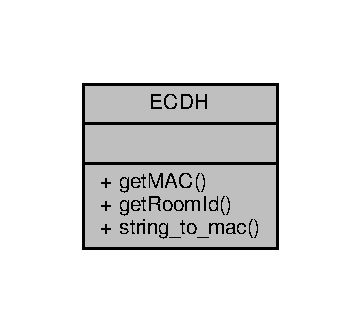
\includegraphics[width=173pt]{classECDH__coll__graph}
\end{center}
\end{figure}
\subsection*{Public Member Functions}
\begin{DoxyCompactItemize}
\item 
uint64\+\_\+t \hyperlink{classECDH_a3ff5f397f1198e2f1daa7689434f338c}{get\+M\+AC} (char $\ast$server\+Request)
\begin{DoxyCompactList}\small\item\em This Function gets the M\+A\+C-\/address from the server request and changes it to an int (the way the M\+A\+C-\/address is stored in the db). \end{DoxyCompactList}\item 
int \hyperlink{classECDH_ac552676079ed12da22501ead4d15500b}{get\+Room\+Id} (uint64\+\_\+t M\+AC)
\begin{DoxyCompactList}\small\item\em Gets the room id from the db. \end{DoxyCompactList}\item 
uint64\+\_\+t \hyperlink{classECDH_a0b5fb1d5817ba51fe4e055190c3c88f2}{string\+\_\+to\+\_\+mac} (std\+::string const \&s)
\begin{DoxyCompactList}\small\item\em This Function turns the M\+A\+C-\/address into an int (the way the M\+A\+C-\/address is stored in the db). \end{DoxyCompactList}\end{DoxyCompactItemize}


\subsection{Member Function Documentation}
\mbox{\Hypertarget{classECDH_a3ff5f397f1198e2f1daa7689434f338c}\label{classECDH_a3ff5f397f1198e2f1daa7689434f338c}} 
\index{E\+C\+DH@{E\+C\+DH}!get\+M\+AC@{get\+M\+AC}}
\index{get\+M\+AC@{get\+M\+AC}!E\+C\+DH@{E\+C\+DH}}
\subsubsection{\texorpdfstring{get\+M\+A\+C()}{getMAC()}}
{\footnotesize\ttfamily uint64\+\_\+t E\+C\+D\+H\+::get\+M\+AC (\begin{DoxyParamCaption}\item[{char $\ast$}]{server\+Request }\end{DoxyParamCaption})}



This Function gets the M\+A\+C-\/address from the server request and changes it to an int (the way the M\+A\+C-\/address is stored in the db). 

\begin{DoxyReturn}{Returns}
The M\+A\+C-\/address in database form. 
\end{DoxyReturn}
\begin{DoxyAuthor}{Author}
Rick Overhorst 
\end{DoxyAuthor}
\mbox{\Hypertarget{classECDH_ac552676079ed12da22501ead4d15500b}\label{classECDH_ac552676079ed12da22501ead4d15500b}} 
\index{E\+C\+DH@{E\+C\+DH}!get\+Room\+Id@{get\+Room\+Id}}
\index{get\+Room\+Id@{get\+Room\+Id}!E\+C\+DH@{E\+C\+DH}}
\subsubsection{\texorpdfstring{get\+Room\+Id()}{getRoomId()}}
{\footnotesize\ttfamily int E\+C\+D\+H\+::get\+Room\+Id (\begin{DoxyParamCaption}\item[{uint64\+\_\+t}]{M\+AC }\end{DoxyParamCaption})}



Gets the room id from the db. 

\begin{DoxyReturn}{Returns}
The room Id. 
\end{DoxyReturn}
\begin{DoxyAuthor}{Author}
Rick Overhorst 
\end{DoxyAuthor}
\mbox{\Hypertarget{classECDH_a0b5fb1d5817ba51fe4e055190c3c88f2}\label{classECDH_a0b5fb1d5817ba51fe4e055190c3c88f2}} 
\index{E\+C\+DH@{E\+C\+DH}!string\+\_\+to\+\_\+mac@{string\+\_\+to\+\_\+mac}}
\index{string\+\_\+to\+\_\+mac@{string\+\_\+to\+\_\+mac}!E\+C\+DH@{E\+C\+DH}}
\subsubsection{\texorpdfstring{string\+\_\+to\+\_\+mac()}{string\_to\_mac()}}
{\footnotesize\ttfamily uint64\+\_\+t E\+C\+D\+H\+::string\+\_\+to\+\_\+mac (\begin{DoxyParamCaption}\item[{std\+::string const \&}]{s }\end{DoxyParamCaption})}



This Function turns the M\+A\+C-\/address into an int (the way the M\+A\+C-\/address is stored in the db). 

\begin{DoxyReturn}{Returns}
The M\+A\+C-\/address in database form. 
\end{DoxyReturn}
\begin{DoxyAuthor}{Author}
Maxim Egorushkin 
\end{DoxyAuthor}


The documentation for this class was generated from the following files\+:\begin{DoxyCompactItemize}
\item 
/home/rso16/projects/\+E\+C\+D\+S/src/\+E\+C\+D\+H/\hyperlink{ECDH_8h}{E\+C\+D\+H.\+h}\item 
/home/rso16/projects/\+E\+C\+D\+S/src/\+E\+C\+D\+H/\hyperlink{ECDH_8cpp}{E\+C\+D\+H.\+cpp}\end{DoxyCompactItemize}

\hypertarget{classMysqlHandler}{}\section{Mysql\+Handler Class Reference}
\label{classMysqlHandler}\index{Mysql\+Handler@{Mysql\+Handler}}


{\ttfamily \#include $<$Mysql\+Handler.\+h$>$}



Collaboration diagram for Mysql\+Handler\+:\nopagebreak
\begin{figure}[H]
\begin{center}
\leavevmode
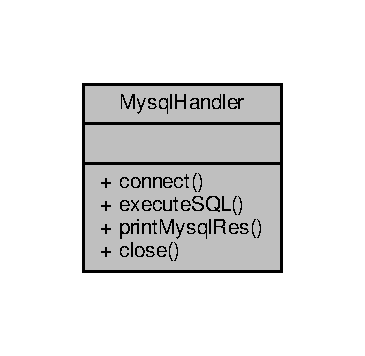
\includegraphics[width=175pt]{classMysqlHandler__coll__graph}
\end{center}
\end{figure}
\subsection*{Public Member Functions}
\begin{DoxyCompactItemize}
\item 
int \hyperlink{classMysqlHandler_acd74d4ee6a2853d07218cd7a300ee6d2}{connect} (char $\ast$\hyperlink{main_8h_afd1a82c786509e03b540bae82af2c137}{server}, char $\ast$user, char $\ast$pass, char $\ast$db\+\_\+name)
\item 
M\+Y\+S\+Q\+L\+\_\+\+R\+ES \hyperlink{classMysqlHandler_abee4d47196df8c42420fe771508a6ff9}{execute\+S\+QL} (char $\ast$sql)
\item 
int \hyperlink{classMysqlHandler_affb80fba704894dca83d563f6582edc0}{print\+Mysql\+Res} (M\+Y\+S\+Q\+L\+\_\+\+R\+ES $\ast$res\+\_\+set)
\item 
int \hyperlink{classMysqlHandler_aef277d872eb51db9ce2fe66fed348941}{close} ()
\end{DoxyCompactItemize}


\subsection{Member Function Documentation}
\mbox{\Hypertarget{classMysqlHandler_aef277d872eb51db9ce2fe66fed348941}\label{classMysqlHandler_aef277d872eb51db9ce2fe66fed348941}} 
\index{Mysql\+Handler@{Mysql\+Handler}!close@{close}}
\index{close@{close}!Mysql\+Handler@{Mysql\+Handler}}
\subsubsection{\texorpdfstring{close()}{close()}}
{\footnotesize\ttfamily int Mysql\+Handler\+::close (\begin{DoxyParamCaption}{ }\end{DoxyParamCaption})}

\mbox{\Hypertarget{classMysqlHandler_acd74d4ee6a2853d07218cd7a300ee6d2}\label{classMysqlHandler_acd74d4ee6a2853d07218cd7a300ee6d2}} 
\index{Mysql\+Handler@{Mysql\+Handler}!connect@{connect}}
\index{connect@{connect}!Mysql\+Handler@{Mysql\+Handler}}
\subsubsection{\texorpdfstring{connect()}{connect()}}
{\footnotesize\ttfamily int Mysql\+Handler\+::connect (\begin{DoxyParamCaption}\item[{char $\ast$}]{server,  }\item[{char $\ast$}]{user,  }\item[{char $\ast$}]{pass,  }\item[{char $\ast$}]{db\+\_\+name }\end{DoxyParamCaption})}

\mbox{\Hypertarget{classMysqlHandler_abee4d47196df8c42420fe771508a6ff9}\label{classMysqlHandler_abee4d47196df8c42420fe771508a6ff9}} 
\index{Mysql\+Handler@{Mysql\+Handler}!execute\+S\+QL@{execute\+S\+QL}}
\index{execute\+S\+QL@{execute\+S\+QL}!Mysql\+Handler@{Mysql\+Handler}}
\subsubsection{\texorpdfstring{execute\+S\+Q\+L()}{executeSQL()}}
{\footnotesize\ttfamily M\+Y\+S\+Q\+L\+\_\+\+R\+ES Mysql\+Handler\+::execute\+S\+QL (\begin{DoxyParamCaption}\item[{char $\ast$}]{sql }\end{DoxyParamCaption})}

\mbox{\Hypertarget{classMysqlHandler_affb80fba704894dca83d563f6582edc0}\label{classMysqlHandler_affb80fba704894dca83d563f6582edc0}} 
\index{Mysql\+Handler@{Mysql\+Handler}!print\+Mysql\+Res@{print\+Mysql\+Res}}
\index{print\+Mysql\+Res@{print\+Mysql\+Res}!Mysql\+Handler@{Mysql\+Handler}}
\subsubsection{\texorpdfstring{print\+Mysql\+Res()}{printMysqlRes()}}
{\footnotesize\ttfamily int Mysql\+Handler\+::print\+Mysql\+Res (\begin{DoxyParamCaption}\item[{M\+Y\+S\+Q\+L\+\_\+\+R\+ES $\ast$}]{res\+\_\+set }\end{DoxyParamCaption})}



The documentation for this class was generated from the following files\+:\begin{DoxyCompactItemize}
\item 
/home/rso16/projects/\+E\+C\+D\+S/src/\+Mysql\+Handler/\hyperlink{MysqlHandler_8h}{Mysql\+Handler.\+h}\item 
/home/rso16/projects/\+E\+C\+D\+S/src/\+Mysql\+Handler/\hyperlink{MysqlHandler_8cpp}{Mysql\+Handler.\+cpp}\end{DoxyCompactItemize}

\hypertarget{classServer}{}\section{Server Class Reference}
\label{classServer}\index{Server@{Server}}


{\ttfamily \#include $<$Server.\+h$>$}



Collaboration diagram for Server\+:\nopagebreak
\begin{figure}[H]
\begin{center}
\leavevmode
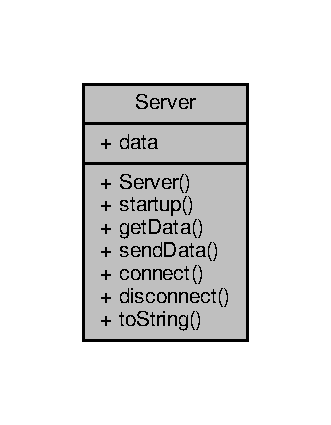
\includegraphics[width=159pt]{classServer__coll__graph}
\end{center}
\end{figure}
\subsection*{Public Member Functions}
\begin{DoxyCompactItemize}
\item 
\hyperlink{classServer_a693b9b86cd9538ff4833a550515cabf8}{Server} (int port=80, char $\ast$ip\+\_\+addr=(char $\ast$) \char`\"{}localhost\char`\"{})
\begin{DoxyCompactList}\small\item\em \hyperlink{classServer}{Server} Constructor. \end{DoxyCompactList}\item 
void \hyperlink{classServer_aaa7517710dd809ba4d965eb83801fd05}{startup} ()
\begin{DoxyCompactList}\small\item\em starts the server \end{DoxyCompactList}\item 
char $\ast$ \hyperlink{classServer_a6b6c39b02aeae611dcb2a9f2f5a8d801}{get\+Data} ()
\begin{DoxyCompactList}\small\item\em Gets the data send by the client/module. \end{DoxyCompactList}\item 
void \hyperlink{classServer_a5061ce779b01e1c5cf8146022db8b08d}{send\+Data} (char $\ast$\hyperlink{classServer_a511bae2c5604c196eb714c798fdf709d}{data})
\begin{DoxyCompactList}\small\item\em Sends the data to the client/module. \end{DoxyCompactList}\item 
void \hyperlink{classServer_a0bd7069e79b4d5268f0947079e1af54a}{connect} ()
\begin{DoxyCompactList}\small\item\em connects the server \end{DoxyCompactList}\item 
void \hyperlink{classServer_acd0114484495cfd2749816ddb12e4246}{disconnect} ()
\begin{DoxyCompactList}\small\item\em disconnects the connection \end{DoxyCompactList}\item 
char $\ast$ \hyperlink{classServer_aee9a13517df765d3c085fab605f24be4}{to\+String} ()
\begin{DoxyCompactList}\small\item\em Gets the ip address. \end{DoxyCompactList}\end{DoxyCompactItemize}
\subsection*{Public Attributes}
\begin{DoxyCompactItemize}
\item 
char \hyperlink{classServer_a511bae2c5604c196eb714c798fdf709d}{data} \mbox{[}100\mbox{]}
\end{DoxyCompactItemize}


\subsection{Constructor \& Destructor Documentation}
\mbox{\Hypertarget{classServer_a693b9b86cd9538ff4833a550515cabf8}\label{classServer_a693b9b86cd9538ff4833a550515cabf8}} 
\index{Server@{Server}!Server@{Server}}
\index{Server@{Server}!Server@{Server}}
\subsubsection{\texorpdfstring{Server()}{Server()}}
{\footnotesize\ttfamily Server\+::\+Server (\begin{DoxyParamCaption}\item[{int}]{port = {\ttfamily 80},  }\item[{char $\ast$}]{ip\+\_\+addr = {\ttfamily (char~$\ast$)~\char`\"{}localhost\char`\"{}} }\end{DoxyParamCaption})}



\hyperlink{classServer}{Server} Constructor. 

\begin{DoxyReturn}{Returns}
none 
\end{DoxyReturn}
\begin{DoxyAuthor}{Author}
Kevin Jansen 
\end{DoxyAuthor}


\subsection{Member Function Documentation}
\mbox{\Hypertarget{classServer_a0bd7069e79b4d5268f0947079e1af54a}\label{classServer_a0bd7069e79b4d5268f0947079e1af54a}} 
\index{Server@{Server}!connect@{connect}}
\index{connect@{connect}!Server@{Server}}
\subsubsection{\texorpdfstring{connect()}{connect()}}
{\footnotesize\ttfamily void Server\+::connect (\begin{DoxyParamCaption}{ }\end{DoxyParamCaption})}



connects the server 

\begin{DoxyReturn}{Returns}
none 
\end{DoxyReturn}
\begin{DoxyAuthor}{Author}
Kevin Jansen 
\end{DoxyAuthor}
\mbox{\Hypertarget{classServer_acd0114484495cfd2749816ddb12e4246}\label{classServer_acd0114484495cfd2749816ddb12e4246}} 
\index{Server@{Server}!disconnect@{disconnect}}
\index{disconnect@{disconnect}!Server@{Server}}
\subsubsection{\texorpdfstring{disconnect()}{disconnect()}}
{\footnotesize\ttfamily void Server\+::disconnect (\begin{DoxyParamCaption}{ }\end{DoxyParamCaption})}



disconnects the connection 

\begin{DoxyReturn}{Returns}
none 
\end{DoxyReturn}
\begin{DoxyAuthor}{Author}
Kevin Jansen 
\end{DoxyAuthor}
\mbox{\Hypertarget{classServer_a6b6c39b02aeae611dcb2a9f2f5a8d801}\label{classServer_a6b6c39b02aeae611dcb2a9f2f5a8d801}} 
\index{Server@{Server}!get\+Data@{get\+Data}}
\index{get\+Data@{get\+Data}!Server@{Server}}
\subsubsection{\texorpdfstring{get\+Data()}{getData()}}
{\footnotesize\ttfamily char $\ast$ Server\+::get\+Data (\begin{DoxyParamCaption}{ }\end{DoxyParamCaption})}



Gets the data send by the client/module. 

\begin{DoxyReturn}{Returns}
The data revieved 
\end{DoxyReturn}
\begin{DoxyAuthor}{Author}
Kevin Jansen 
\end{DoxyAuthor}
\mbox{\Hypertarget{classServer_a5061ce779b01e1c5cf8146022db8b08d}\label{classServer_a5061ce779b01e1c5cf8146022db8b08d}} 
\index{Server@{Server}!send\+Data@{send\+Data}}
\index{send\+Data@{send\+Data}!Server@{Server}}
\subsubsection{\texorpdfstring{send\+Data()}{sendData()}}
{\footnotesize\ttfamily void Server\+::send\+Data (\begin{DoxyParamCaption}\item[{char $\ast$}]{data }\end{DoxyParamCaption})}



Sends the data to the client/module. 

\begin{DoxyReturn}{Returns}
none 
\end{DoxyReturn}
\begin{DoxyAuthor}{Author}
Kevin Jansen 
\end{DoxyAuthor}
\mbox{\Hypertarget{classServer_aaa7517710dd809ba4d965eb83801fd05}\label{classServer_aaa7517710dd809ba4d965eb83801fd05}} 
\index{Server@{Server}!startup@{startup}}
\index{startup@{startup}!Server@{Server}}
\subsubsection{\texorpdfstring{startup()}{startup()}}
{\footnotesize\ttfamily void Server\+::startup (\begin{DoxyParamCaption}{ }\end{DoxyParamCaption})}



starts the server 

\begin{DoxyReturn}{Returns}
none 
\end{DoxyReturn}
\begin{DoxyAuthor}{Author}
Kevin Jansen 
\end{DoxyAuthor}
\mbox{\Hypertarget{classServer_aee9a13517df765d3c085fab605f24be4}\label{classServer_aee9a13517df765d3c085fab605f24be4}} 
\index{Server@{Server}!to\+String@{to\+String}}
\index{to\+String@{to\+String}!Server@{Server}}
\subsubsection{\texorpdfstring{to\+String()}{toString()}}
{\footnotesize\ttfamily char $\ast$ Server\+::to\+String (\begin{DoxyParamCaption}{ }\end{DoxyParamCaption})}



Gets the ip address. 

\begin{DoxyReturn}{Returns}
The ip address 
\end{DoxyReturn}
\begin{DoxyAuthor}{Author}
Kevin Jansen 
\end{DoxyAuthor}


\subsection{Member Data Documentation}
\mbox{\Hypertarget{classServer_a511bae2c5604c196eb714c798fdf709d}\label{classServer_a511bae2c5604c196eb714c798fdf709d}} 
\index{Server@{Server}!data@{data}}
\index{data@{data}!Server@{Server}}
\subsubsection{\texorpdfstring{data}{data}}
{\footnotesize\ttfamily char Server\+::data\mbox{[}100\mbox{]}}



The documentation for this class was generated from the following files\+:\begin{DoxyCompactItemize}
\item 
/home/rso16/projects/\+E\+C\+D\+S/src/\+Server/\hyperlink{Server_8h}{Server.\+h}\item 
/home/rso16/projects/\+E\+C\+D\+S/src/\+Server/\hyperlink{Server_8cpp}{Server.\+cpp}\end{DoxyCompactItemize}

\chapter{File Documentation}
\hypertarget{CurlHandler_8cpp}{}\section{/home/rso16/projects/\+E\+C\+D\+S/src/\+Curl\+Handler/\+Curl\+Handler.cpp File Reference}
\label{CurlHandler_8cpp}\index{/home/rso16/projects/\+E\+C\+D\+S/src/\+Curl\+Handler/\+Curl\+Handler.\+cpp@{/home/rso16/projects/\+E\+C\+D\+S/src/\+Curl\+Handler/\+Curl\+Handler.\+cpp}}
{\ttfamily \#include \char`\"{}Curl\+Handler.\+h\char`\"{}}\newline
Include dependency graph for Curl\+Handler.\+cpp\+:\nopagebreak
\begin{figure}[H]
\begin{center}
\leavevmode
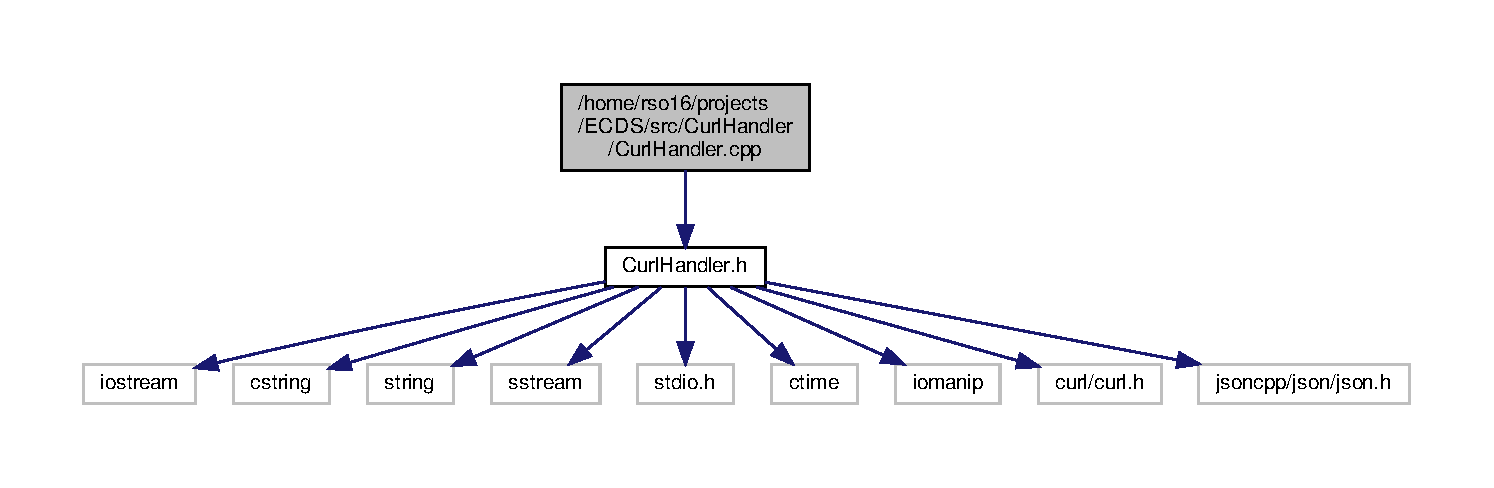
\includegraphics[width=350pt]{CurlHandler_8cpp__incl}
\end{center}
\end{figure}

\hypertarget{CurlHandler_8h}{}\section{/home/rso16/projects/\+E\+C\+D\+S/src/\+Curl\+Handler/\+Curl\+Handler.h File Reference}
\label{CurlHandler_8h}\index{/home/rso16/projects/\+E\+C\+D\+S/src/\+Curl\+Handler/\+Curl\+Handler.\+h@{/home/rso16/projects/\+E\+C\+D\+S/src/\+Curl\+Handler/\+Curl\+Handler.\+h}}
{\ttfamily \#include $<$iostream$>$}\newline
{\ttfamily \#include $<$cstring$>$}\newline
{\ttfamily \#include $<$string$>$}\newline
{\ttfamily \#include $<$sstream$>$}\newline
{\ttfamily \#include $<$stdio.\+h$>$}\newline
{\ttfamily \#include $<$ctime$>$}\newline
{\ttfamily \#include $<$iomanip$>$}\newline
{\ttfamily \#include $<$curl/curl.\+h$>$}\newline
{\ttfamily \#include $<$jsoncpp/json/json.\+h$>$}\newline
Include dependency graph for Curl\+Handler.\+h\+:\nopagebreak
\begin{figure}[H]
\begin{center}
\leavevmode
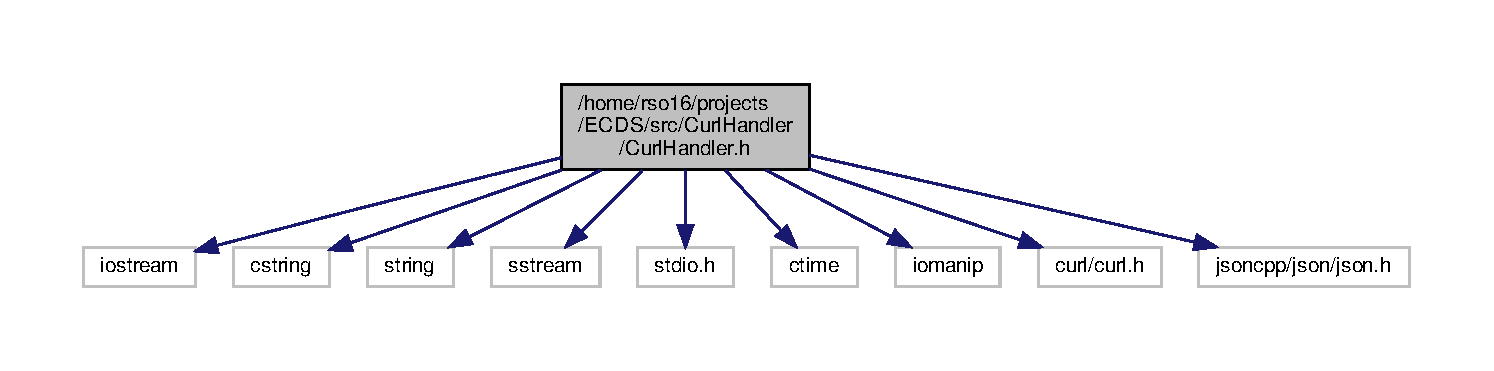
\includegraphics[width=350pt]{CurlHandler_8h__incl}
\end{center}
\end{figure}
This graph shows which files directly or indirectly include this file\+:\nopagebreak
\begin{figure}[H]
\begin{center}
\leavevmode
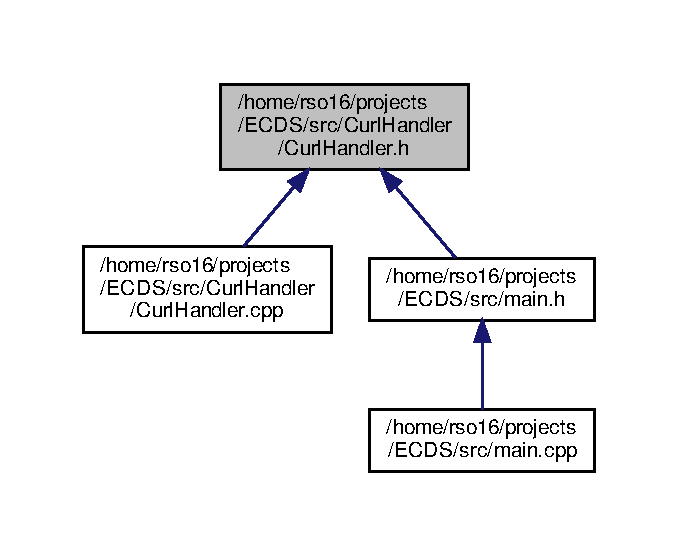
\includegraphics[width=326pt]{CurlHandler_8h__dep__incl}
\end{center}
\end{figure}
\subsection*{Classes}
\begin{DoxyCompactItemize}
\item 
class \hyperlink{classCurlHandler}{Curl\+Handler}
\end{DoxyCompactItemize}
\subsection*{Macros}
\begin{DoxyCompactItemize}
\item 
\#define \hyperlink{CurlHandler_8h_a6b20d41d6252e9871430c242cb1a56e7}{B\+U\+F\+F\+E\+R\+\_\+\+S\+I\+ZE}~500
\end{DoxyCompactItemize}
\subsection*{Variables}
\begin{DoxyCompactItemize}
\item 
const std\+::string \hyperlink{CurlHandler_8h_ad924492dcf12a127180c2c9b8918939b}{Base\+U\+RL} = \char`\"{}https\+://roostertest.\+windesheim.\+nl/Web\+Untis/Timetable.\+do?request.\+prevent\+Cache=1543327601812\&\char`\"{}
\item 
const std\+::string \hyperlink{CurlHandler_8h_a690460d365a25ec4f0dd7b69c23dfbb6}{Request\+Class\+Data} = \char`\"{}ajax\+Command=get\+Weekly\+Timetable\&element\+Type=4\&department\+Id=0\&filter\+Id=2\&\char`\"{}
\end{DoxyCompactItemize}


\subsection{Macro Definition Documentation}
\mbox{\Hypertarget{CurlHandler_8h_a6b20d41d6252e9871430c242cb1a56e7}\label{CurlHandler_8h_a6b20d41d6252e9871430c242cb1a56e7}} 
\index{Curl\+Handler.\+h@{Curl\+Handler.\+h}!B\+U\+F\+F\+E\+R\+\_\+\+S\+I\+ZE@{B\+U\+F\+F\+E\+R\+\_\+\+S\+I\+ZE}}
\index{B\+U\+F\+F\+E\+R\+\_\+\+S\+I\+ZE@{B\+U\+F\+F\+E\+R\+\_\+\+S\+I\+ZE}!Curl\+Handler.\+h@{Curl\+Handler.\+h}}
\subsubsection{\texorpdfstring{B\+U\+F\+F\+E\+R\+\_\+\+S\+I\+ZE}{BUFFER\_SIZE}}
{\footnotesize\ttfamily \#define B\+U\+F\+F\+E\+R\+\_\+\+S\+I\+ZE~500}



\subsection{Variable Documentation}
\mbox{\Hypertarget{CurlHandler_8h_ad924492dcf12a127180c2c9b8918939b}\label{CurlHandler_8h_ad924492dcf12a127180c2c9b8918939b}} 
\index{Curl\+Handler.\+h@{Curl\+Handler.\+h}!Base\+U\+RL@{Base\+U\+RL}}
\index{Base\+U\+RL@{Base\+U\+RL}!Curl\+Handler.\+h@{Curl\+Handler.\+h}}
\subsubsection{\texorpdfstring{Base\+U\+RL}{BaseURL}}
{\footnotesize\ttfamily const std\+::string Base\+U\+RL = \char`\"{}https\+://roostertest.\+windesheim.\+nl/Web\+Untis/Timetable.\+do?request.\+prevent\+Cache=1543327601812\&\char`\"{}}

\mbox{\Hypertarget{CurlHandler_8h_a690460d365a25ec4f0dd7b69c23dfbb6}\label{CurlHandler_8h_a690460d365a25ec4f0dd7b69c23dfbb6}} 
\index{Curl\+Handler.\+h@{Curl\+Handler.\+h}!Request\+Class\+Data@{Request\+Class\+Data}}
\index{Request\+Class\+Data@{Request\+Class\+Data}!Curl\+Handler.\+h@{Curl\+Handler.\+h}}
\subsubsection{\texorpdfstring{Request\+Class\+Data}{RequestClassData}}
{\footnotesize\ttfamily const std\+::string Request\+Class\+Data = \char`\"{}ajax\+Command=get\+Weekly\+Timetable\&element\+Type=4\&department\+Id=0\&filter\+Id=2\&\char`\"{}}


\hypertarget{ECDH_8cpp}{}\section{/home/rso16/projects/\+E\+C\+D\+S/src/\+E\+C\+D\+H/\+E\+C\+DH.cpp File Reference}
\label{ECDH_8cpp}\index{/home/rso16/projects/\+E\+C\+D\+S/src/\+E\+C\+D\+H/\+E\+C\+D\+H.\+cpp@{/home/rso16/projects/\+E\+C\+D\+S/src/\+E\+C\+D\+H/\+E\+C\+D\+H.\+cpp}}
{\ttfamily \#include \char`\"{}E\+C\+D\+H.\+h\char`\"{}}\newline
Include dependency graph for E\+C\+D\+H.\+cpp\+:\nopagebreak
\begin{figure}[H]
\begin{center}
\leavevmode
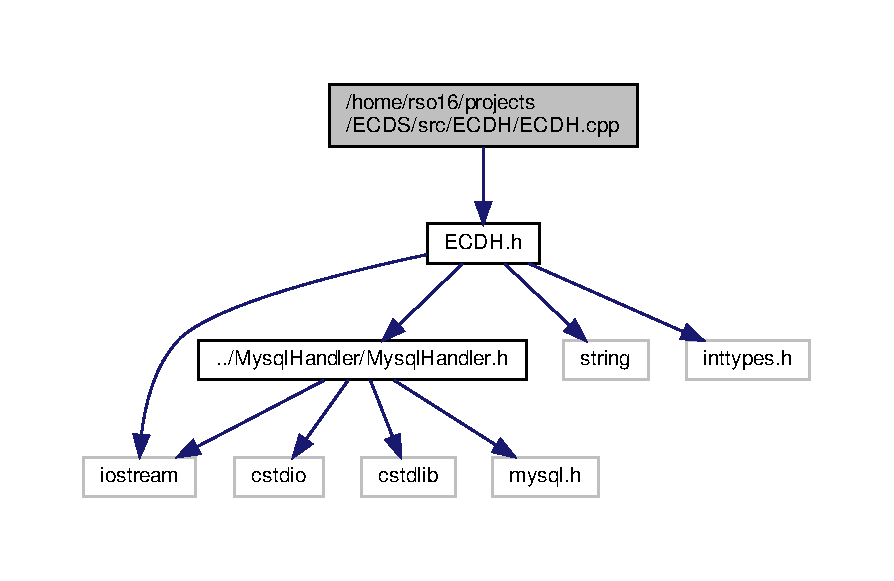
\includegraphics[width=350pt]{ECDH_8cpp__incl}
\end{center}
\end{figure}

\hypertarget{ECDH_8h}{}\section{/home/rso16/projects/\+E\+C\+D\+S/src/\+E\+C\+D\+H/\+E\+C\+DH.h File Reference}
\label{ECDH_8h}\index{/home/rso16/projects/\+E\+C\+D\+S/src/\+E\+C\+D\+H/\+E\+C\+D\+H.\+h@{/home/rso16/projects/\+E\+C\+D\+S/src/\+E\+C\+D\+H/\+E\+C\+D\+H.\+h}}
{\ttfamily \#include \char`\"{}../\+Mysql\+Handler/\+Mysql\+Handler.\+h\char`\"{}}\newline
{\ttfamily \#include $<$iostream$>$}\newline
{\ttfamily \#include $<$string$>$}\newline
{\ttfamily \#include $<$inttypes.\+h$>$}\newline
Include dependency graph for E\+C\+D\+H.\+h\+:
% FIG 0
This graph shows which files directly or indirectly include this file\+:
% FIG 1
\subsection*{Classes}
\begin{DoxyCompactItemize}
\item 
class \hyperlink{classECDH}{E\+C\+DH}
\end{DoxyCompactItemize}
\subsection*{Macros}
\begin{DoxyCompactItemize}
\item 
\#define \hyperlink{ECDH_8h_a01caa36caf53c1930566778551deb453}{B\+E\+G\+I\+N\+\_\+\+O\+F\+\_\+\+M\+AC}~0
\item 
\#define \hyperlink{ECDH_8h_a4c987156ced719bbcf398ab6c76289c0}{M\+A\+C\+\_\+\+S\+I\+ZE}~17
\item 
\#define \hyperlink{ECDH_8h_a0421e684a5689f5f219dd56f237356ed}{S\+Q\+L\+\_\+\+S\+I\+ZE}~53
\item 
\#define \hyperlink{ECDH_8h_a2201ea1dbd502467d7aa23f70a59752c}{S\+Q\+L\+\_\+\+S\+TM}~\char`\"{}select R\+ID from Boards where M\+AC = \char`\"{}
\item 
\#define \hyperlink{ECDH_8h_aacbb9e1f38be71e22df1584a37c56693}{\+\_\+\+\_\+\+S\+T\+D\+C\+\_\+\+F\+O\+R\+M\+A\+T\+\_\+\+M\+A\+C\+R\+OS}
\item 
\#define \hyperlink{ECDH_8h_ac3652ebcb3bd5c77a3734d4a30e8bfdf}{P\+I\+\_\+\+B\+OX}~0
\item 
\#define \hyperlink{ECDH_8h_afcb894f39b5abbf1a913067f9e3af4e5}{U\+\_\+\+B\+OX}~1
\item 
\#define \hyperlink{ECDH_8h_a23a390cc01279924f6190334c5fa97a0}{B\+OX}~\hyperlink{ECDH_8h_afcb894f39b5abbf1a913067f9e3af4e5}{U\+\_\+\+B\+OX}
\item 
\#define \hyperlink{ECDH_8h_a24cd3c37a165a8c4626d9e78df4574ff}{S\+E\+R\+V\+ER}~\char`\"{}localhost\char`\"{}
\item 
\#define \hyperlink{ECDH_8h_a8bfbbf31b7d3c07215440d18a064b7f4}{U\+S\+ER}~\char`\"{}root\char`\"{}
\item 
\#define \hyperlink{ECDH_8h_a9e8538fad4eee548302ad9f60e6d47ca}{P\+A\+S\+S\+W\+O\+RD}~\char`\"{}\char`\"{}
\item 
\#define \hyperlink{ECDH_8h_a39dc88d73783e112dbfcf98adbdbefa6}{D\+A\+T\+A\+B\+A\+SE}~\char`\"{}windesheim\char`\"{}
\end{DoxyCompactItemize}


\subsection{Macro Definition Documentation}
\mbox{\Hypertarget{ECDH_8h_aacbb9e1f38be71e22df1584a37c56693}\label{ECDH_8h_aacbb9e1f38be71e22df1584a37c56693}} 
\index{E\+C\+D\+H.\+h@{E\+C\+D\+H.\+h}!\+\_\+\+\_\+\+S\+T\+D\+C\+\_\+\+F\+O\+R\+M\+A\+T\+\_\+\+M\+A\+C\+R\+OS@{\+\_\+\+\_\+\+S\+T\+D\+C\+\_\+\+F\+O\+R\+M\+A\+T\+\_\+\+M\+A\+C\+R\+OS}}
\index{\+\_\+\+\_\+\+S\+T\+D\+C\+\_\+\+F\+O\+R\+M\+A\+T\+\_\+\+M\+A\+C\+R\+OS@{\+\_\+\+\_\+\+S\+T\+D\+C\+\_\+\+F\+O\+R\+M\+A\+T\+\_\+\+M\+A\+C\+R\+OS}!E\+C\+D\+H.\+h@{E\+C\+D\+H.\+h}}
\subsubsection{\texorpdfstring{\+\_\+\+\_\+\+S\+T\+D\+C\+\_\+\+F\+O\+R\+M\+A\+T\+\_\+\+M\+A\+C\+R\+OS}{\_\_STDC\_FORMAT\_MACROS}}
{\footnotesize\ttfamily \#define \+\_\+\+\_\+\+S\+T\+D\+C\+\_\+\+F\+O\+R\+M\+A\+T\+\_\+\+M\+A\+C\+R\+OS}

\mbox{\Hypertarget{ECDH_8h_a01caa36caf53c1930566778551deb453}\label{ECDH_8h_a01caa36caf53c1930566778551deb453}} 
\index{E\+C\+D\+H.\+h@{E\+C\+D\+H.\+h}!B\+E\+G\+I\+N\+\_\+\+O\+F\+\_\+\+M\+AC@{B\+E\+G\+I\+N\+\_\+\+O\+F\+\_\+\+M\+AC}}
\index{B\+E\+G\+I\+N\+\_\+\+O\+F\+\_\+\+M\+AC@{B\+E\+G\+I\+N\+\_\+\+O\+F\+\_\+\+M\+AC}!E\+C\+D\+H.\+h@{E\+C\+D\+H.\+h}}
\subsubsection{\texorpdfstring{B\+E\+G\+I\+N\+\_\+\+O\+F\+\_\+\+M\+AC}{BEGIN\_OF\_MAC}}
{\footnotesize\ttfamily \#define B\+E\+G\+I\+N\+\_\+\+O\+F\+\_\+\+M\+AC~0}

\mbox{\Hypertarget{ECDH_8h_a23a390cc01279924f6190334c5fa97a0}\label{ECDH_8h_a23a390cc01279924f6190334c5fa97a0}} 
\index{E\+C\+D\+H.\+h@{E\+C\+D\+H.\+h}!B\+OX@{B\+OX}}
\index{B\+OX@{B\+OX}!E\+C\+D\+H.\+h@{E\+C\+D\+H.\+h}}
\subsubsection{\texorpdfstring{B\+OX}{BOX}}
{\footnotesize\ttfamily \#define B\+OX~\hyperlink{ECDH_8h_afcb894f39b5abbf1a913067f9e3af4e5}{U\+\_\+\+B\+OX}}

\mbox{\Hypertarget{ECDH_8h_a39dc88d73783e112dbfcf98adbdbefa6}\label{ECDH_8h_a39dc88d73783e112dbfcf98adbdbefa6}} 
\index{E\+C\+D\+H.\+h@{E\+C\+D\+H.\+h}!D\+A\+T\+A\+B\+A\+SE@{D\+A\+T\+A\+B\+A\+SE}}
\index{D\+A\+T\+A\+B\+A\+SE@{D\+A\+T\+A\+B\+A\+SE}!E\+C\+D\+H.\+h@{E\+C\+D\+H.\+h}}
\subsubsection{\texorpdfstring{D\+A\+T\+A\+B\+A\+SE}{DATABASE}}
{\footnotesize\ttfamily \#define D\+A\+T\+A\+B\+A\+SE~\char`\"{}windesheim\char`\"{}}

\mbox{\Hypertarget{ECDH_8h_a4c987156ced719bbcf398ab6c76289c0}\label{ECDH_8h_a4c987156ced719bbcf398ab6c76289c0}} 
\index{E\+C\+D\+H.\+h@{E\+C\+D\+H.\+h}!M\+A\+C\+\_\+\+S\+I\+ZE@{M\+A\+C\+\_\+\+S\+I\+ZE}}
\index{M\+A\+C\+\_\+\+S\+I\+ZE@{M\+A\+C\+\_\+\+S\+I\+ZE}!E\+C\+D\+H.\+h@{E\+C\+D\+H.\+h}}
\subsubsection{\texorpdfstring{M\+A\+C\+\_\+\+S\+I\+ZE}{MAC\_SIZE}}
{\footnotesize\ttfamily \#define M\+A\+C\+\_\+\+S\+I\+ZE~17}

\mbox{\Hypertarget{ECDH_8h_a9e8538fad4eee548302ad9f60e6d47ca}\label{ECDH_8h_a9e8538fad4eee548302ad9f60e6d47ca}} 
\index{E\+C\+D\+H.\+h@{E\+C\+D\+H.\+h}!P\+A\+S\+S\+W\+O\+RD@{P\+A\+S\+S\+W\+O\+RD}}
\index{P\+A\+S\+S\+W\+O\+RD@{P\+A\+S\+S\+W\+O\+RD}!E\+C\+D\+H.\+h@{E\+C\+D\+H.\+h}}
\subsubsection{\texorpdfstring{P\+A\+S\+S\+W\+O\+RD}{PASSWORD}}
{\footnotesize\ttfamily \#define P\+A\+S\+S\+W\+O\+RD~\char`\"{}\char`\"{}}

\mbox{\Hypertarget{ECDH_8h_ac3652ebcb3bd5c77a3734d4a30e8bfdf}\label{ECDH_8h_ac3652ebcb3bd5c77a3734d4a30e8bfdf}} 
\index{E\+C\+D\+H.\+h@{E\+C\+D\+H.\+h}!P\+I\+\_\+\+B\+OX@{P\+I\+\_\+\+B\+OX}}
\index{P\+I\+\_\+\+B\+OX@{P\+I\+\_\+\+B\+OX}!E\+C\+D\+H.\+h@{E\+C\+D\+H.\+h}}
\subsubsection{\texorpdfstring{P\+I\+\_\+\+B\+OX}{PI\_BOX}}
{\footnotesize\ttfamily \#define P\+I\+\_\+\+B\+OX~0}

\mbox{\Hypertarget{ECDH_8h_a24cd3c37a165a8c4626d9e78df4574ff}\label{ECDH_8h_a24cd3c37a165a8c4626d9e78df4574ff}} 
\index{E\+C\+D\+H.\+h@{E\+C\+D\+H.\+h}!S\+E\+R\+V\+ER@{S\+E\+R\+V\+ER}}
\index{S\+E\+R\+V\+ER@{S\+E\+R\+V\+ER}!E\+C\+D\+H.\+h@{E\+C\+D\+H.\+h}}
\subsubsection{\texorpdfstring{S\+E\+R\+V\+ER}{SERVER}}
{\footnotesize\ttfamily \#define S\+E\+R\+V\+ER~\char`\"{}localhost\char`\"{}}

\mbox{\Hypertarget{ECDH_8h_a0421e684a5689f5f219dd56f237356ed}\label{ECDH_8h_a0421e684a5689f5f219dd56f237356ed}} 
\index{E\+C\+D\+H.\+h@{E\+C\+D\+H.\+h}!S\+Q\+L\+\_\+\+S\+I\+ZE@{S\+Q\+L\+\_\+\+S\+I\+ZE}}
\index{S\+Q\+L\+\_\+\+S\+I\+ZE@{S\+Q\+L\+\_\+\+S\+I\+ZE}!E\+C\+D\+H.\+h@{E\+C\+D\+H.\+h}}
\subsubsection{\texorpdfstring{S\+Q\+L\+\_\+\+S\+I\+ZE}{SQL\_SIZE}}
{\footnotesize\ttfamily \#define S\+Q\+L\+\_\+\+S\+I\+ZE~53}

\mbox{\Hypertarget{ECDH_8h_a2201ea1dbd502467d7aa23f70a59752c}\label{ECDH_8h_a2201ea1dbd502467d7aa23f70a59752c}} 
\index{E\+C\+D\+H.\+h@{E\+C\+D\+H.\+h}!S\+Q\+L\+\_\+\+S\+TM@{S\+Q\+L\+\_\+\+S\+TM}}
\index{S\+Q\+L\+\_\+\+S\+TM@{S\+Q\+L\+\_\+\+S\+TM}!E\+C\+D\+H.\+h@{E\+C\+D\+H.\+h}}
\subsubsection{\texorpdfstring{S\+Q\+L\+\_\+\+S\+TM}{SQL\_STM}}
{\footnotesize\ttfamily \#define S\+Q\+L\+\_\+\+S\+TM~\char`\"{}select R\+ID from Boards where M\+AC = \char`\"{}}

\mbox{\Hypertarget{ECDH_8h_afcb894f39b5abbf1a913067f9e3af4e5}\label{ECDH_8h_afcb894f39b5abbf1a913067f9e3af4e5}} 
\index{E\+C\+D\+H.\+h@{E\+C\+D\+H.\+h}!U\+\_\+\+B\+OX@{U\+\_\+\+B\+OX}}
\index{U\+\_\+\+B\+OX@{U\+\_\+\+B\+OX}!E\+C\+D\+H.\+h@{E\+C\+D\+H.\+h}}
\subsubsection{\texorpdfstring{U\+\_\+\+B\+OX}{U\_BOX}}
{\footnotesize\ttfamily \#define U\+\_\+\+B\+OX~1}

\mbox{\Hypertarget{ECDH_8h_a8bfbbf31b7d3c07215440d18a064b7f4}\label{ECDH_8h_a8bfbbf31b7d3c07215440d18a064b7f4}} 
\index{E\+C\+D\+H.\+h@{E\+C\+D\+H.\+h}!U\+S\+ER@{U\+S\+ER}}
\index{U\+S\+ER@{U\+S\+ER}!E\+C\+D\+H.\+h@{E\+C\+D\+H.\+h}}
\subsubsection{\texorpdfstring{U\+S\+ER}{USER}}
{\footnotesize\ttfamily \#define U\+S\+ER~\char`\"{}root\char`\"{}}


\hypertarget{main_8cpp}{}\section{/home/rso16/projects/\+E\+C\+D\+S/src/main.cpp File Reference}
\label{main_8cpp}\index{/home/rso16/projects/\+E\+C\+D\+S/src/main.\+cpp@{/home/rso16/projects/\+E\+C\+D\+S/src/main.\+cpp}}
{\ttfamily \#include \char`\"{}main.\+h\char`\"{}}\newline
Include dependency graph for main.\+cpp\+:
% FIG 0
\subsection*{Functions}
\begin{DoxyCompactItemize}
\item 
int \hyperlink{main_8cpp_ac0f2228420376f4db7e1274f2b41667c}{main} (int argc, const char $\ast$argv\mbox{[}$\,$\mbox{]})
\end{DoxyCompactItemize}


\subsection{Function Documentation}
\mbox{\Hypertarget{main_8cpp_ac0f2228420376f4db7e1274f2b41667c}\label{main_8cpp_ac0f2228420376f4db7e1274f2b41667c}} 
\index{main.\+cpp@{main.\+cpp}!main@{main}}
\index{main@{main}!main.\+cpp@{main.\+cpp}}
\subsubsection{\texorpdfstring{main()}{main()}}
{\footnotesize\ttfamily int main (\begin{DoxyParamCaption}\item[{int}]{argc,  }\item[{const char $\ast$}]{argv\mbox{[}$\,$\mbox{]} }\end{DoxyParamCaption})}


\hypertarget{main_8h}{}\section{/home/rso16/projects/\+E\+C\+D\+S/src/main.h File Reference}
\label{main_8h}\index{/home/rso16/projects/\+E\+C\+D\+S/src/main.\+h@{/home/rso16/projects/\+E\+C\+D\+S/src/main.\+h}}
{\ttfamily \#include $<$stdio.\+h$>$}\newline
{\ttfamily \#include \char`\"{}Server/\+Server.\+h\char`\"{}}\newline
{\ttfamily \#include $<$stdlib.\+h$>$}\newline
{\ttfamily \#include $<$unistd.\+h$>$}\newline
{\ttfamily \#include $<$string.\+h$>$}\newline
{\ttfamily \#include \char`\"{}Mysql\+Handler/\+Mysql\+Handler.\+h\char`\"{}}\newline
{\ttfamily \#include \char`\"{}E\+C\+D\+H/\+E\+C\+D\+H.\+h\char`\"{}}\newline
{\ttfamily \#include \char`\"{}Curl\+Handler/\+Curl\+Handler.\+h\char`\"{}}\newline
Include dependency graph for main.\+h\+:\nopagebreak
\begin{figure}[H]
\begin{center}
\leavevmode
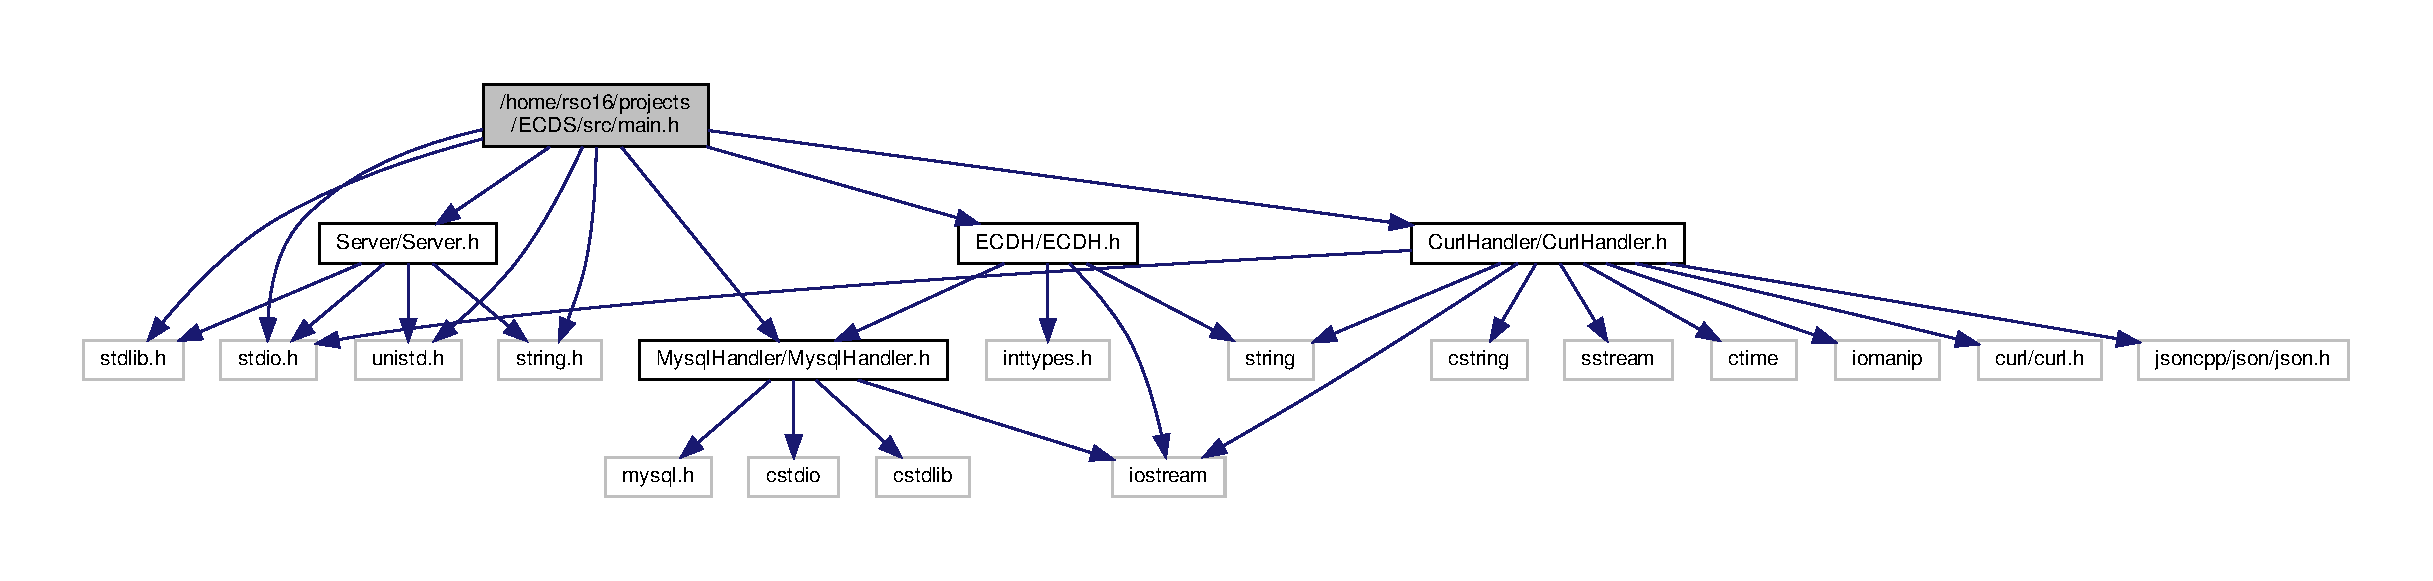
\includegraphics[width=350pt]{main_8h__incl}
\end{center}
\end{figure}
This graph shows which files directly or indirectly include this file\+:\nopagebreak
\begin{figure}[H]
\begin{center}
\leavevmode
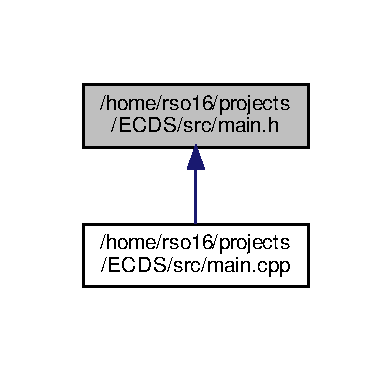
\includegraphics[width=188pt]{main_8h__dep__incl}
\end{center}
\end{figure}
\subsection*{Functions}
\begin{DoxyCompactItemize}
\item 
int \hyperlink{main_8h_ac0f2228420376f4db7e1274f2b41667c}{main} (int argc, const char $\ast$argv\mbox{[}$\,$\mbox{]})
\end{DoxyCompactItemize}
\subsection*{Variables}
\begin{DoxyCompactItemize}
\item 
\hyperlink{classMysqlHandler}{Mysql\+Handler} \hyperlink{main_8h_a52c8376765d7847a2347ff9e77249f32}{m\+Handler}
\item 
\hyperlink{classECDH}{E\+C\+DH} \hyperlink{main_8h_adde9b3824c73385d6da28d4707dddc09}{e\+Handler}
\item 
\hyperlink{classServer}{Server} \hyperlink{main_8h_afd1a82c786509e03b540bae82af2c137}{server}
\item 
\hyperlink{classCurlHandler}{Curl\+Handler} \hyperlink{main_8h_a0c3f11694a4ac69a68e2ca62b8fc48a5}{c\+Handler}
\end{DoxyCompactItemize}


\subsection{Function Documentation}
\mbox{\Hypertarget{main_8h_ac0f2228420376f4db7e1274f2b41667c}\label{main_8h_ac0f2228420376f4db7e1274f2b41667c}} 
\index{main.\+h@{main.\+h}!main@{main}}
\index{main@{main}!main.\+h@{main.\+h}}
\subsubsection{\texorpdfstring{main()}{main()}}
{\footnotesize\ttfamily int main (\begin{DoxyParamCaption}\item[{int}]{argc,  }\item[{const char $\ast$}]{argv\mbox{[}$\,$\mbox{]} }\end{DoxyParamCaption})}



\subsection{Variable Documentation}
\mbox{\Hypertarget{main_8h_a0c3f11694a4ac69a68e2ca62b8fc48a5}\label{main_8h_a0c3f11694a4ac69a68e2ca62b8fc48a5}} 
\index{main.\+h@{main.\+h}!c\+Handler@{c\+Handler}}
\index{c\+Handler@{c\+Handler}!main.\+h@{main.\+h}}
\subsubsection{\texorpdfstring{c\+Handler}{cHandler}}
{\footnotesize\ttfamily \hyperlink{classCurlHandler}{Curl\+Handler} c\+Handler}

\mbox{\Hypertarget{main_8h_adde9b3824c73385d6da28d4707dddc09}\label{main_8h_adde9b3824c73385d6da28d4707dddc09}} 
\index{main.\+h@{main.\+h}!e\+Handler@{e\+Handler}}
\index{e\+Handler@{e\+Handler}!main.\+h@{main.\+h}}
\subsubsection{\texorpdfstring{e\+Handler}{eHandler}}
{\footnotesize\ttfamily \hyperlink{classECDH}{E\+C\+DH} e\+Handler}

\mbox{\Hypertarget{main_8h_a52c8376765d7847a2347ff9e77249f32}\label{main_8h_a52c8376765d7847a2347ff9e77249f32}} 
\index{main.\+h@{main.\+h}!m\+Handler@{m\+Handler}}
\index{m\+Handler@{m\+Handler}!main.\+h@{main.\+h}}
\subsubsection{\texorpdfstring{m\+Handler}{mHandler}}
{\footnotesize\ttfamily \hyperlink{classMysqlHandler}{Mysql\+Handler} m\+Handler}

\mbox{\Hypertarget{main_8h_afd1a82c786509e03b540bae82af2c137}\label{main_8h_afd1a82c786509e03b540bae82af2c137}} 
\index{main.\+h@{main.\+h}!server@{server}}
\index{server@{server}!main.\+h@{main.\+h}}
\subsubsection{\texorpdfstring{server}{server}}
{\footnotesize\ttfamily \hyperlink{classServer}{Server} server}


\hypertarget{MysqlHandler_8cpp}{}\section{/home/rso16/projects/\+E\+C\+D\+S/src/\+Mysql\+Handler/\+Mysql\+Handler.cpp File Reference}
\label{MysqlHandler_8cpp}\index{/home/rso16/projects/\+E\+C\+D\+S/src/\+Mysql\+Handler/\+Mysql\+Handler.\+cpp@{/home/rso16/projects/\+E\+C\+D\+S/src/\+Mysql\+Handler/\+Mysql\+Handler.\+cpp}}
{\ttfamily \#include \char`\"{}Mysql\+Handler.\+h\char`\"{}}\newline
Include dependency graph for Mysql\+Handler.\+cpp\+:\nopagebreak
\begin{figure}[H]
\begin{center}
\leavevmode
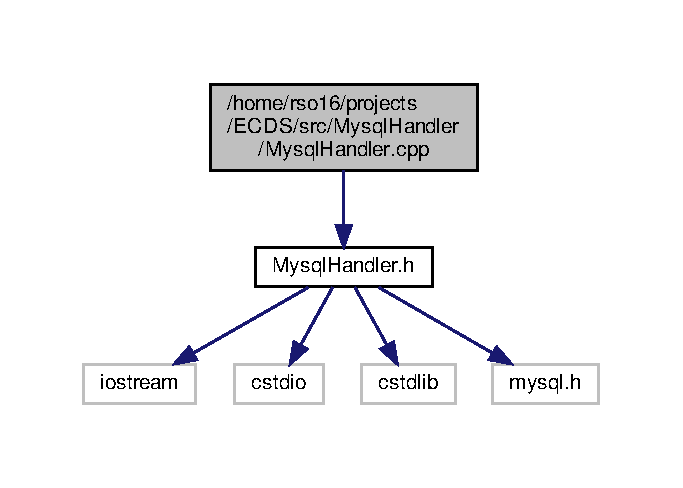
\includegraphics[width=328pt]{MysqlHandler_8cpp__incl}
\end{center}
\end{figure}

\hypertarget{MysqlHandler_8h}{}\section{/home/rso16/projects/\+E\+C\+D\+S/src/\+Mysql\+Handler/\+Mysql\+Handler.h File Reference}
\label{MysqlHandler_8h}\index{/home/rso16/projects/\+E\+C\+D\+S/src/\+Mysql\+Handler/\+Mysql\+Handler.\+h@{/home/rso16/projects/\+E\+C\+D\+S/src/\+Mysql\+Handler/\+Mysql\+Handler.\+h}}
{\ttfamily \#include $<$iostream$>$}\newline
{\ttfamily \#include $<$cstdio$>$}\newline
{\ttfamily \#include $<$cstdlib$>$}\newline
{\ttfamily \#include $<$mysql.\+h$>$}\newline
Include dependency graph for Mysql\+Handler.\+h\+:\nopagebreak
\begin{figure}[H]
\begin{center}
\leavevmode
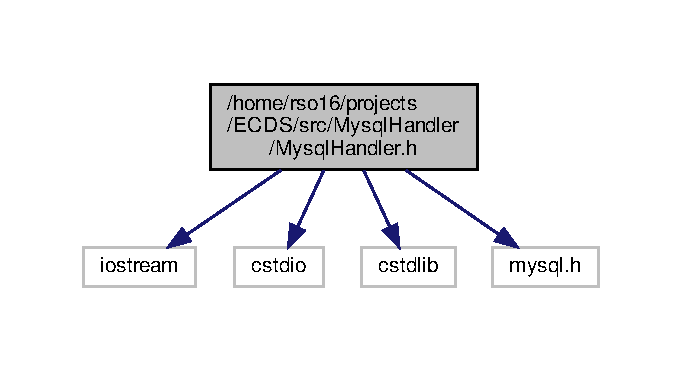
\includegraphics[width=328pt]{MysqlHandler_8h__incl}
\end{center}
\end{figure}
This graph shows which files directly or indirectly include this file\+:\nopagebreak
\begin{figure}[H]
\begin{center}
\leavevmode
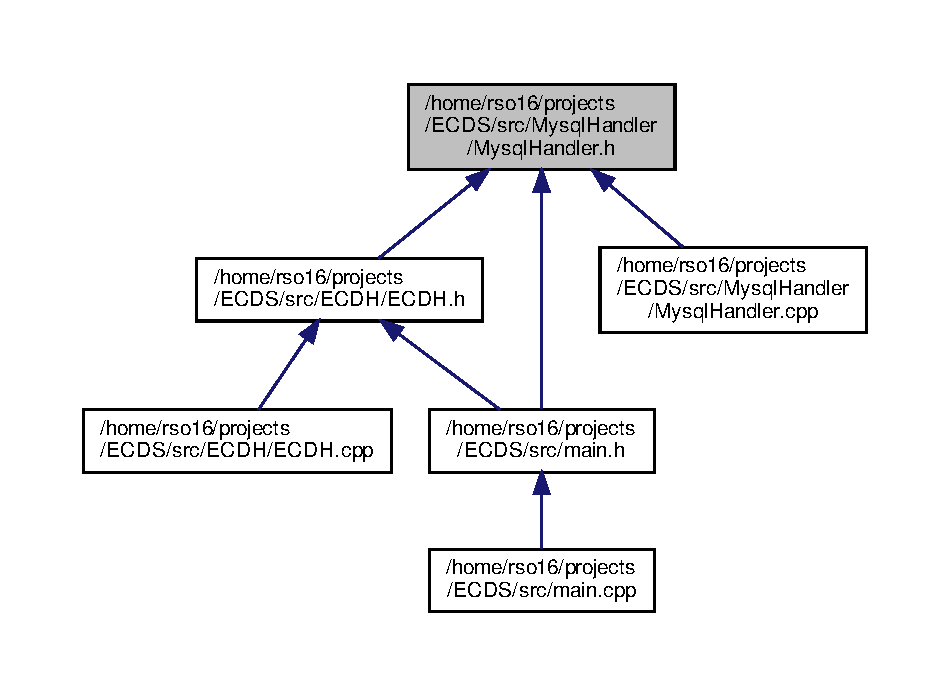
\includegraphics[width=350pt]{MysqlHandler_8h__dep__incl}
\end{center}
\end{figure}
\subsection*{Classes}
\begin{DoxyCompactItemize}
\item 
class \hyperlink{classMysqlHandler}{Mysql\+Handler}
\end{DoxyCompactItemize}

\hypertarget{Server_8cpp}{}\section{/home/rso16/projects/\+E\+C\+D\+S/src/\+Server/\+Server.cpp File Reference}
\label{Server_8cpp}\index{/home/rso16/projects/\+E\+C\+D\+S/src/\+Server/\+Server.\+cpp@{/home/rso16/projects/\+E\+C\+D\+S/src/\+Server/\+Server.\+cpp}}
{\ttfamily \#include \char`\"{}Server.\+h\char`\"{}}\newline
Include dependency graph for Server.\+cpp\+:\nopagebreak
\begin{figure}[H]
\begin{center}
\leavevmode
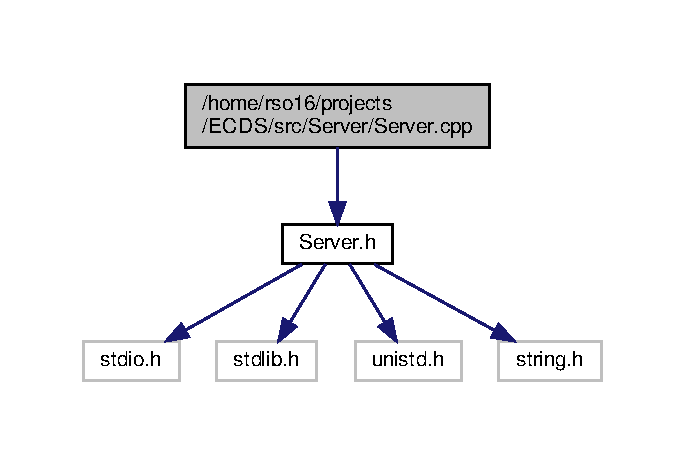
\includegraphics[width=329pt]{Server_8cpp__incl}
\end{center}
\end{figure}

\hypertarget{Server_8h}{}\section{/home/rso16/projects/\+E\+C\+D\+S/src/\+Server/\+Server.h File Reference}
\label{Server_8h}\index{/home/rso16/projects/\+E\+C\+D\+S/src/\+Server/\+Server.\+h@{/home/rso16/projects/\+E\+C\+D\+S/src/\+Server/\+Server.\+h}}
{\ttfamily \#include $<$stdio.\+h$>$}\newline
{\ttfamily \#include $<$stdlib.\+h$>$}\newline
{\ttfamily \#include $<$unistd.\+h$>$}\newline
{\ttfamily \#include $<$string.\+h$>$}\newline
Include dependency graph for Server.\+h\+:
% FIG 0
This graph shows which files directly or indirectly include this file\+:
% FIG 1
\subsection*{Classes}
\begin{DoxyCompactItemize}
\item 
class \hyperlink{classServer}{Server}
\end{DoxyCompactItemize}

%--- End generated contents ---

% Index
\backmatter
\newpage
\phantomsection
\clearemptydoublepage
\addcontentsline{toc}{chapter}{Index}
\printindex

\end{document}
